\chapter{Experimentation Methodolgy}\label{ch:method}

The NFCTP is the first attempt at solving the supply and demand of the nuclear
fuel cycle in a dynamic manner within a NFC simulation. Accordingly, there is no
precedent for investigating the performance and efficacy of a given
approach. This chapter describes one such novel approach in which rules for
generating instances of exchanges are defined, exchanges are generated,
exchanges are executed, and results are analyzed. 

The chapter begins with a discussion of the generation of exchanges, in \S
\ref{method:setup}. Two types of exchanges are included: one in which reactors
are requesting fuel, and one in which reactors are supplying used fuel. In NFC
parlance, these are called the \textit{Front End} of the fuel cycle and
\textit{Back End} of the fuel cycle. Notably, both of these exchanges can occur
in the same time step. \S \ref{method:setup:split} describes how a full exchange
may be split into multiple exchanges for any given time step. 

Generating and solving instances of exchanges at a large scale is a difficult
problem. The Cyclopts (Cyclus Optimization Studies) framework was implemented
for this purpose. Cyclopts has both a Python and C layer. The Python layer is
largely responsible for generating exchanges and interfacing with an associated
persistence mechanism. The C layer is linked agaisnt the Cyclus kernel shared
object library and is responsible for calling directly into the kernel's
resource exchange API. \S \ref{method:tools} describes the implementation of
Cyclopts and its varied modes of operation. 

\section{Generating Exchanges}\label{method:setup}

This section focuses on two distinct \textit{species} of exchanges, those
related to the \textit{front end} of the nuclear fuel cycle and those related to
the \textit{back end} of the nuclear fuel cycle. Broadly, the front end of the
fuel cycle is concerned with fueling reactors, and the back end is concerned
with either recycling or disposing of used fuel exiting reactors. 

\S \ref{abm:dre}, however, only discusseses the methodology for solving a single
exchange. Therefore, an argument must be made for why it is possible to split a
single exchange into multiple exchanges, and specifically why that is valid in
the case of the front and back ends of the NFC. Such an argument is made in \S
\ref{method:setup:split}.

Exchange generation is defined by two types parameters, \textit{exchange} and
\textit{species} parameters. Exchange parameters apply to any species of
exchange, and species parameters apply to a specific species. \S
\ref{method:setup:params} provides a discussion of exchange parameters. \S
\ref{method:setup:front} and \ref{method:setup:back} then follow with a full
description of modeling assumptions and species parameters included for
generating both species of exchanges.

\subsection{Splitting Exchanges}\label{method:setup:split}

A well known simplification of the Multicommodity Transportation Problem occurs
when supply and demand is separate for separate commodities. The large
multicommodity problem can then be decomposed into $n$ subproblems, where $n$ is
the number of commodities. Each subproblem can be solved separately from the
others.

An analog exists in the NFCTP when the Exchange Graph is \textit{separable}. A
bipartite graph with directed arcs, $A$, consisting of sending nodes, $U$, and
receiving nodes, $V$, is separable if there a partition

\begin{equation}
  A = A_{1} \cup A_{2}
\end{equation}

\begin{equation}
  U = U_{1} \cup U_{2}
\end{equation}

\begin{equation}
  V = V_{1} \cup V_{2}
\end{equation}

such that no node in $U_1$ is connected to a node in $V_2$ and no node in $U_2$
is connected to a node in $V_1$. The graph shown in Figure \ref{fig:basic_part} is an
example of a separable bipartite graph.

\begin{figure}
  \begin{center}
    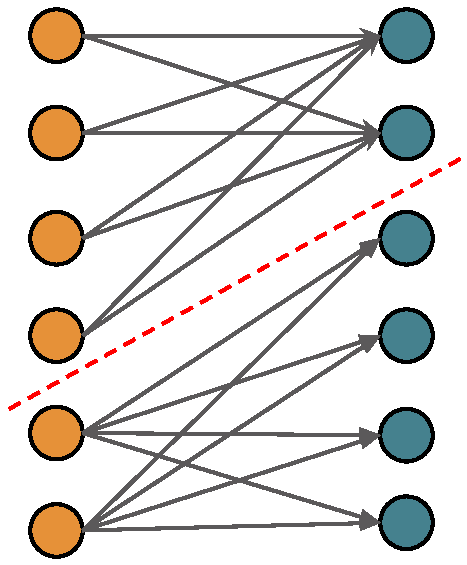
\includegraphics[width=0.55\textwidth]{exchange_part_supreq.pdf}
    \caption[]{
      \label{fig:basic_part}
      A separable bipartite graph with the partition shown as a red 
      dashed line.}
  \end{center}
\end{figure}

The Exchange Graph of the NFCTP, however, has additional structure in the form
of portfolios and thus has a stricter notion of separability. Specifically, the
partition must also separate the set of supplier portfolios, $S$, and requester
portfolios, $R$, as in Equations \ref{eqn:sup_part} and \ref{eqn:req_part},
respectively.

\begin{equation}\label{eqn:sup_part}
  S = S_{1} \cup S_{2}
\end{equation}

\begin{equation}\label{eqn:req_part}
  R = R_{1} \cup R_{2}
\end{equation}

Figure \ref{fig:port_part} depicts a separable Exchange Graph, for example,
while Figure \ref{fig:port_no_part} shows an Exchange Graph that is not
separable, even though the underlying bipartite graph is, due to the lack of a
fully separable portfolio partition.

\begin{figure}
  \begin{center}
    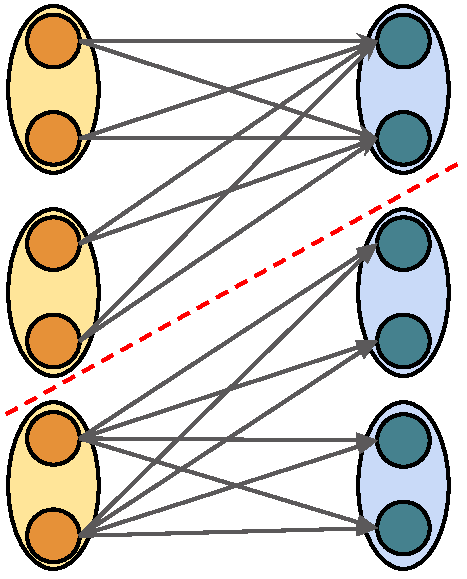
\includegraphics[width=0.55\textwidth]{exchange_part_port.pdf}
    \caption[]{
      \label{fig:port_part}
      A separable Exchange Graph with nodes grouped by portfolio and the
      separating partition shown as a red dashed line.}
  \end{center}
\end{figure}

\begin{figure}
  \begin{center}
    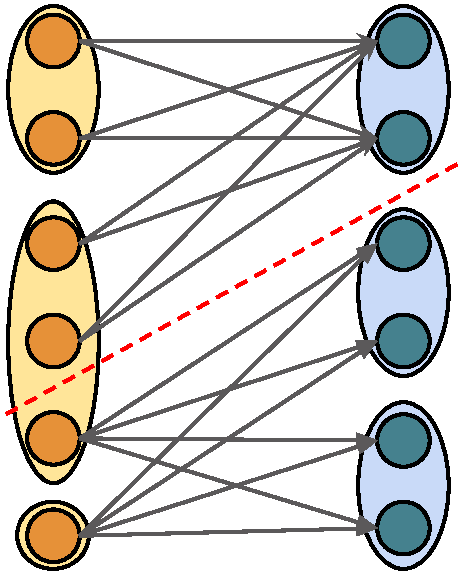
\includegraphics[width=0.55\textwidth]{exchange_no_part_port.pdf}
    \caption[]{
      \label{fig:port_no_part}
      An Exchange Graph with nodes grouped by portfolio that is \textit{not}
      separable because a portfolio crosses the node partition.}
  \end{center}
\end{figure}

The Exchange Graph resulting from the information gathering phase of the DRE
specifically from a NFC application will be minimally separable into front-end
and back-end exchanges if two conditions are met:

\begin{enumerate}
  \item Reactors output commodities can \textit{not} be sent to both other
    reactors and supporting facilities.

  \item Supporting facility output commodities can \textit{not} be sent to both
    other supporting facilities and reactors.
\end{enumerate}



\subsection{Exchange Parameters}\label{method:setup:params}

\subsection{Front-End Exchanges}\label{method:setup:front}

\subsection{Back-End Exchanges}\label{method:setup:back}

\section{Experimental Tools}\label{method:tools}

\subsection{Structure}\label{method:tools:struc}

\subsection{Persistence Mechanisms}\label{method:tools:hdf5}

what gets recorded

\subsection{High Throughput Computing}\label{method:tools:htc}

Things \cite{bui_work_2011}.
